\documentclass[]{article}

\usepackage[T1]{fontenc}
\usepackage[utf8]{inputenc}
\usepackage{amsthm, amsmath, amsfonts}
\usepackage{blkarray}
\usepackage{bigstrut}
\usepackage{graphicx}

\newcommand{\avaliacao}{2}
\newcommand{\disciplina}{Probabilidade e Estatística}
\newcommand{\semestre}{2024/1}


\theoremstyle{definition}
\newtheorem{ex}{Exercício}

\renewcommand{\SS}{\mathcal{S}}

\begin{document}
\thispagestyle{empty}
\begin{center}
\Large{\avaliacao ª Avaliação de \disciplina\ - \semestre}

\large{Prof. Dr. Alessandro José Queiroz Sarnaglia}
\end{center}

\begin{ex}
Suponha que 70\% de todos os motoristas parem completamente num cruzamento com semáforo vermelho quando não há outros carros à vista.
\begin{enumerate}
	\item Se 10 motoristas são observados, qual a probabilidade de exatamente a metade parar completamente?
	\item Se 10 motoristas são observados, qual a probabilidade de no mínimo a metade parar totalmente?
	\item Se fossem 100 motoristas, qual a probabilidade aproximada de no mínimo a metade parar completamente?
\end{enumerate}
\end{ex}


\begin{ex}
Um casal decide ter filhos até ter duas meninas ($F$). Assumindo $P(F) = 0.5$, responda:
\begin{enumerate}
	\item Quantos meninos o casal deve esperar ter?
	\item Qual é a probabilidade de o casal ter ao menos dois meninos?
\end{enumerate}
\end{ex}


\begin{ex}
A vida útil de um equipamento segue a distribuição lognormal com $\mu=3.0$ e $\sigma = 0.5$.
\begin{enumerate}
	\item Qual é o valor da média e o desvio padrão da vida útil?
	\item Qual é a probabilidade da vida útil ser no máximo 50?
\end{enumerate}
\end{ex}

\begin{ex}
Determinado evento ocorre em um ponto $(X,Y)$ na região ilustrada abaixo. Suponha que nenhum ponto é privilegiado para a ocorrência do evento.
\begin{enumerate}
	\item Encontre as fdp's marginais de $X$ e $Y$.
	\item Encontre $\text{Cov}(X,Y)$.
	\item As vac's $X$ e $Y$ são independentes? Justifique!
\end{enumerate}
\begin{center}
	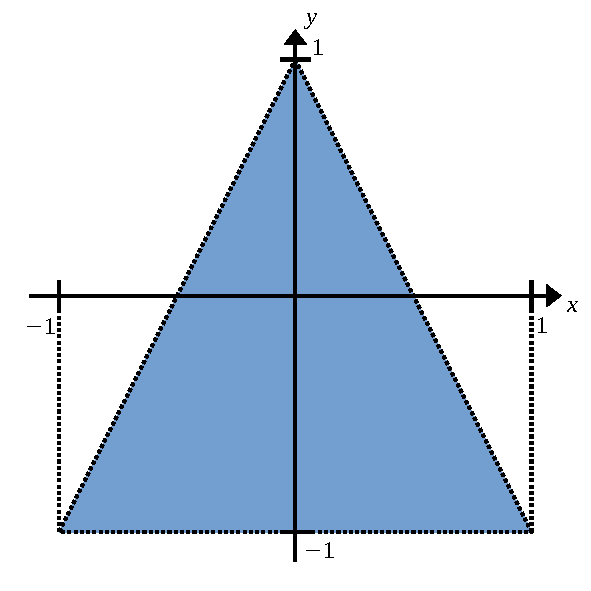
\includegraphics[width=0.45\linewidth]{figura_substitutiva_2}
\end{center}
\end{ex}


\end{document}
